\documentclass{article}
%\documentclass[a4paper,landscape]{article}

\usepackage{graphicx}
\usepackage{tabularx}
\usepackage{adjustbox}
\usepackage{amsmath}
\usepackage{amsfonts}
\usepackage{multirow}

%% Key definitions for text elements. USE THEM
\def\secref#1{Sec.~\ref{#1}}
\def\figref#1{Fig.~\ref{#1}}
\def\tabref#1{Tab.~\ref{#1}}
\def\eqref#1{Eq.~(\ref{#1})}
\def\algref#1{Alg.~\ref{#1}}
\def\appref#1{App.~\ref{#1}}

\newcommand\etal{\emph{et al.}}

\usepackage{rotating}

\usepackage{amsopn}


\newcommand{\bJidx}[1]{\ensuremath{\mathbf{J}^{[#1]}}}
\newcommand{\cose}{\mathrm{cose}}
\newcommand{\bzidx}[1]{\mathbf{z}^{[{#1}]}}
\newcommand{\bxidx}[1]{\mathbf{x}^{[{#1}]}}
\newcommand{\bhidx}[1]{\mathbf{h}^{[{#1}]}}
\newcommand{\bOmegaidx}[1]{\mathbf{\Omega}^{[{#1}]}}
\newcommand{\bSigmaidx}[1]{\mathbf{\Sigma}^{[{#1}]}}
\newcommand{\bHidx}[1]{\mathbf{H}^{[{#1}]}}

\newcommand{\bv}{\mathbf{v}}
\newcommand{\bl}{\mathbf{l}}
\newcommand{\bt}{\mathbf{t}}
\newcommand{\bo}{\mathbf{o}}
\newcommand{\bM}{\mathbf{M}}
\newcommand{\bL}{\mathbf{L}}
\newcommand{\bA}{\mathbf{A}}
\newcommand{\bB}{\mathbf{B}}
\newcommand{\bE}{\mathbf{E}}
\newcommand{\bK}{\mathbf{K}}
\newcommand{\bC}{\mathbf{C}}
\newcommand{\bH}{\mathbf{H}}
\newcommand{\bI}{\mathbf{I}}
\newcommand{\bP}{\mathbf{P}}
\newcommand{\bX}{\mathbf{X}}
\newcommand{\bZ}{\mathbf{Z}}
\newcommand{\bR}{\mathbf{R}}
\newcommand{\bS}{\mathbf{S}}
\newcommand{\bU}{\mathbf{U}}
\newcommand{\bV}{\mathbf{V}}
\newcommand{\bT}{\mathbf{T}}
\newcommand{\bpi}{\mathbf{\pi}}
\newcommand{\btl}{\mathbf{tl}}
\newcommand{\bbr}{\mathbf{br}}


\newcommand{\iD}{\mathbf{D}}
\newcommand{\iN}{\mathbf{N}}
\newcommand{\iI}{\mathbf{I}}

\newcommand\norm[1]{\left\lVert#1\right\rVert}

\newcommand{\bzridx}[1]{\ensuremath{\mathbf{z}^{({#1})}}}
\newcommand{\bxridx}[1]{\mathbf{x}^{({#1})}}
\newcommand{\bhridx}[1]{\mathbf{h}^{({#1})}}

\newcommand{\bJ}{\mathbf{J}}
\newcommand{\bZero}{\mathbf{0}}

\newcommand{\cS}{\mathcal{S}}
\newcommand{\cE}{\mathcal{E}}
\newcommand{\cC}{\mathcal{C}}
\newcommand{\cSM}{\mathcal{SM}}
\newcommand{\cR}{\mathcal{R}}
\newcommand{\cM}{\mathcal{M}}
\newcommand{\cP}{\mathcal{P}}
\newcommand{\cL}{\mathcal{L}}
\newcommand{\cD}{\mathcal{D}}
\newcommand{\cZ}{\mathcal{Z}}
\newcommand{\cX}{\mathcal{X}}
\newcommand{\range}[3]{#1_{#2:#3}}


\newcommand{\ba}{\mathbf{a}}
\newcommand{\bb}{\mathbf{b}}
\newcommand{\bc}{\mathbf{c}}
\newcommand{\bd}{\mathbf{d}}
\newcommand{\be}{\mathbf{e}}
\newcommand{\ec}{\mathbf{e}}
\newcommand{\bm}{\mathbf{m}}
\newcommand{\bg}{\mathbf{g}}
\newcommand{\Dim}{\mathrm{Dim}}

\newcommand{\bs}{\mathbf{s}}
\newcommand{\bx}{\mathbf{x}}
\newcommand{\by}{\mathbf{y}}
\newcommand{\br}{\mathbf{r}}
\newcommand{\bz}{\mathbf{z}}
\newcommand{\bu}{\mathbf{u}}
\newcommand{\bn}{\mathbf{n}}
\newcommand{\bh}{\mathbf{h}}
\newcommand{\bff}{\mathbf{f}}
\newcommand{\bp}{\mathbf{p}}
\newcommand{\bDelta}{\mathbf{\Delta}}
\newcommand{\bGamma}{\mathbf{\Gamma}}
\newcommand{\bDeltaalpha}{\mathbf{\Delta \alpha}}
\newcommand{\bDeltar}{\mathbf{\Delta r}}
\newcommand{\bDeltax}{\mathbf{\Delta x}}
\newcommand{\bDeltaX}{\mathbf{\Delta X}}
\newcommand{\bDeltat}{\mathbf{\Delta t}}
\newcommand{\bDeltaR}{\mathbf{\Delta R}}
\newcommand{\tTov}{\mathrm{t2v}}
\newcommand{\vTot}{\mathrm{v2t}}

\newcommand{\bO}{\mathbf{O}}

\newcommand{\defeq}{=}


\newcommand{\bmu}{\mathbf{\mu}}
\newcommand{\bnu}{\mathbf{\nu}}
\newcommand{\bSigma}{\mathbf{\Sigma}}
\newcommand{\bOmega}{\mathbf{\Omega}}
\newcommand{\bLambda}{\mathbf{\Lambda}}

\newcommand{\mat}[1]{#1}
\newcommand{\mbf}[1]{\mathbf{#1}}
\newcommand{\defn}[1]{\emph{#1}}

\newcommand{\mysum}{\sum}
\newcommand{\myprod}{\prod}
\newcommand{\eq}{=}
\newcommand{\pv}{\mathrm{P}}
%\newcommand{\implies}{\Rightarrow}
\newcommand{\Parents}{\mathrm{Parents}}
\newcommand{\rj}{\mathrm{j}}
\newcommand{\proj}{\mathrm{proj}}
\DeclareMathOperator*{\argmax}{argmax}
\DeclareMathOperator*{\argmin}{argmin}
\DeclareMathOperator*{\atantwo}{atantwo}

\newcommand{\mR}{\mathbb{R}}
\newcommand{\mN}{\mathbb{N}}
\newcommand{\mC}{\mathbb{C}}




%\usepackage{geometry}
%\geometry{
%	a4paper,
%%	total={170mm,257mm},
%	left=0mm,
%	top=0mm,
%	right=0mm,
%	bottom=0mm,
%}

\title{\LARGE \bf Semantic Mapping}

\begin{document}
	
	\maketitle
	
	\section{Introduction}
	
	Acquisition and modeling of semantic information is a key requisite for mobile robots to be deployed in human environments. In this field, fundamental aspects faced by research are: the recognition of places and objects, the construction of semantic models and the exploration strategies to enrich contextual knowledge. 
	
	In this paper, we will present relevant work that focused on the mentioned problems, namely, perception, mapping and exploration, along with our system proposal.

	\subsection{Motivation}
	
	\begin{itemize}
		\item Traditional mapping techniques return a geometric model of the environment that can be used by the robot for computing distances to obstacles or finding paths toward goals.
		\item Manipulation and navigation tasks may require human level knowledge (e.g., objects/places categories, functions, properties, and so on) to be accomplished.
		\item By extracting semantic information from sensory data it's possible to fullfill this requirement.
	\end{itemize}
	
		
	\subsection{Definition}
		
	Semantic mapping:
		
	\begin{itemize}
		\item is the problem of building a model of the environment that allows to share knowledge between humans and robots.
		\item has the function of providing the robot with a representation of the environment for the completion of its tasks.
		\item is a core component of many robotic applications.
	\end{itemize}
		
	\subsection{Building a semantic representation of the environment}
	
	\begin{itemize}
		\item The process of semantic mapping consists in integrating sensor measurements in the robot internal representation of the environment.
		\item The output of visual and range sensors is processed to extract meaningful information for recovering the structure and objects/places categories of the scene.
		\item This information is consecutively used to update the current robot belief about the state of the environment.
	\end{itemize}
	
	\begin{figure}[h]
		\centering
		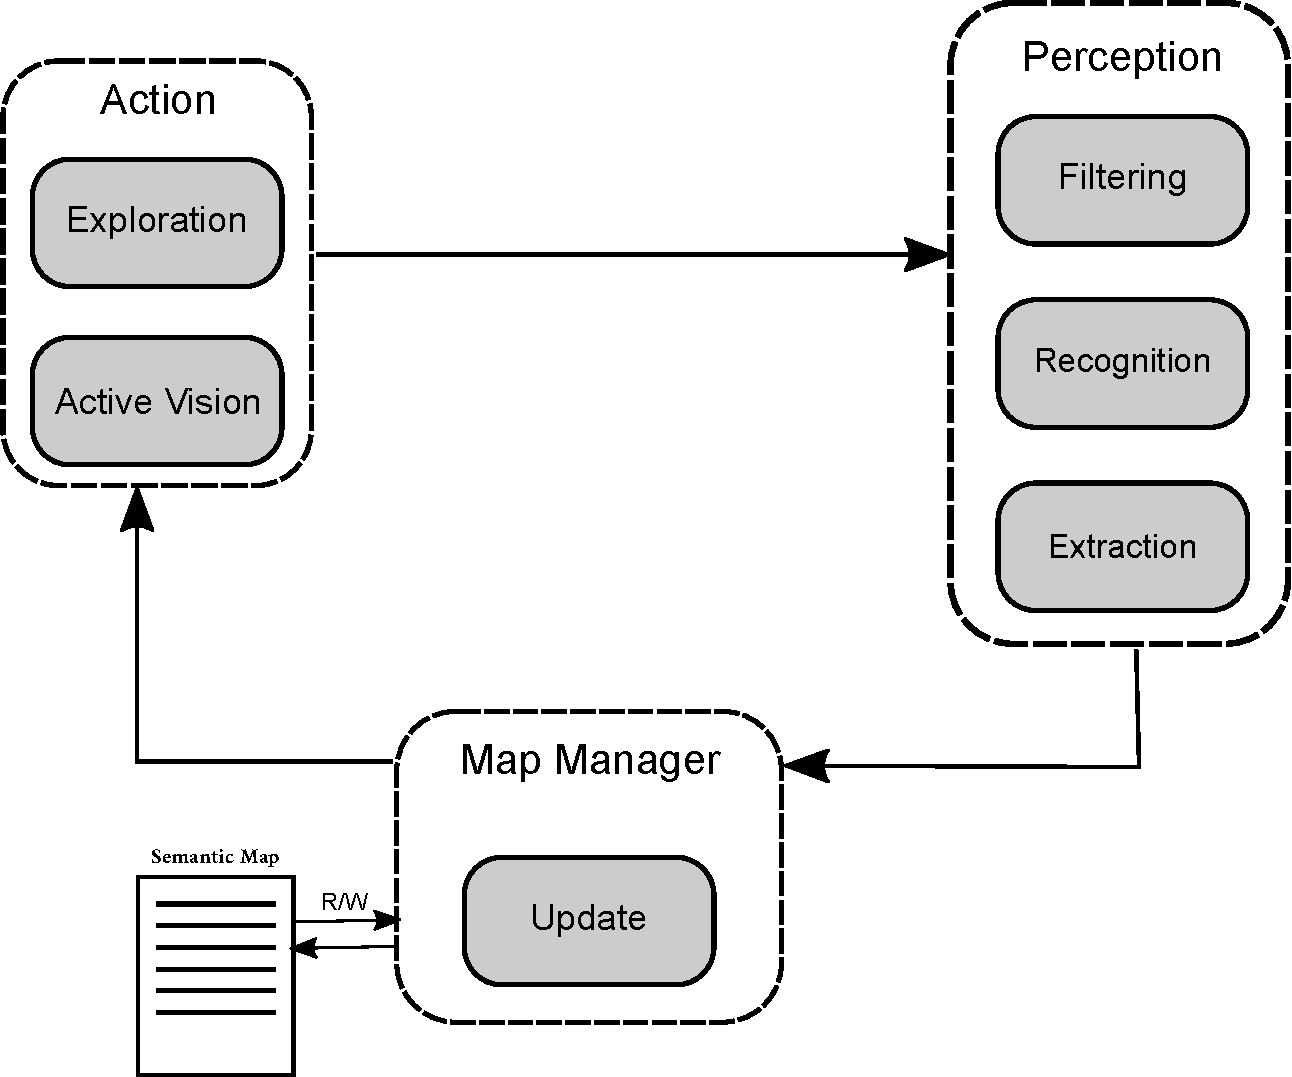
\includegraphics[width=\linewidth]{pics/drawing-crop.pdf}
		\caption{Semantic mapping system.}
		\label{fig:pipeline}
	\end{figure}
	
	\newpage
		
	\section{System Overview}
			
	A semantic map is a triple:
	
	\begin{equation}
	\cSM = < \cR, \cM, \cP >,
	\end{equation}
	
	\noindent
	with:
	
	\begin{itemize}
		\item $\cR$: reference system
		\item $\cM$: metric information obtained from sensors
		\item $\cP$: predicates compliant with basic concept hierarchy.
	\end{itemize}
	
	\subsection{Global Reference System}	
	
	The reference system is used to express all the elements of the map in a single frame.
	
	\subsection{Metric Map}	
	
	The metric information $\cM$ of the semantic map can be seen as a collection of 3D geometric models:
	
	\begin{equation}
	\cM = \{\bM_1 \cdots \bM_N\},
	\end{equation}
	
	\noindent	
	where each model $\bM_i$ is an entity defined by:
	
	\begin{itemize}
		\item {\bf Pose3D}: $\bX = [ \bR | \bt] \in SE(3)$,
		\item {\bf Size3D}: $\bS = <\bL ,\bU> \in \mathbf{R}^3 $,
		\item {\bf Representation3D}: e.g. a point cloud, a mesh and so on.
	\end{itemize}
	
	The adopted convention is that the pose $\bX$ is assumed to refer to the centroid of the model and that the bounding box $\bS$ is defined by two 3D vectors that specify its "lower" and "upper" corners.
	
	\subsection{Property Map}	
	
	The semantic information $\cP$ contains the assertions about the properties of the objects in $\cM$:
	
	\begin{equation}
	\cP = \{\bP_1 \cdots \bP_N\},
	\end{equation}
	
	\noindent
	where each $\bP_i$ is a set of predicates of $arity = (1 \dots q)$ that are instances of $\bm_i$ (corresponding to the geometrical object $\bM_i$).
	
	\subsection{Interface}
	
	Possible operations on the map are:
	
	\begin{itemize}
		\item query for object: given an object it's possible to check if it's already present in the map
		\item update object: allows to update an object present in the map with a new observation
		\item add object: allows to add an object to the map if it's seen for the first time
		\item render map: builds a 3d model from the collection of objects, this function can be used for navigation and visualization.
		\item serialize/deserialize: these functions allow to save a map on disk and to load it for later use.
	\end{itemize}
	
	
	\section{Perception}
	
	The perception module takes every frame coming from the RGB-D camera and has to tell which objects are seen by the robot. This information will be passed to the map manager so to update the robot knowledge of the environment.
	
	\subsection{Approaches}
	
	\begin{itemize}
		\item {\bf Geometric only:} consists in recovering only the geometric structure of the environment.
		\item {\bf Semantic only:} focuses on the extraction of semantic information from sensory data, assuming that no reconstruction is needed.
		\item {\bf Pipelined:} consists in recovering a geometric model of the environment and, subsequently, using this model to extract semantic information.
		\item {\bf Parallel:} in this approach, reconstruction and recognition are performed separately (and simultaneously) and then, their results are fused together by the symbol grounding module.
		\item {\bf Joint:} in this approach, perception is formulated as a problem that jointly estimates geometric structure and semantic properties of the environment. 
	\end{itemize}
	
	\section{Recognition}
	
	Extracting semantic information from visual data is one of the  fundamental problems of computer vision. Recognition can be decomposed into sub-tasks, depending on the information one is interested to extract from the input data. These sub-tasks can be organized on a progression that goes from coarse to fine grained inference.
	
	\subsection{Approaches}
	
	\begin{itemize}
		\item {\bf Image classification:} assigning a semantic label to an input image from a fixed set of categories.
		\item {\bf Object detection:} making a prediction not only of object categories but also of their spatial locations.
		\item {\bf Image segmentation:} finding groups of pixels that possess some "similarity" among each other.
		\item {\bf Scene labeling:} assigning a semantic label to each geometric feature of the scene.
		\item {\bf 3d object recognition:} given an input model and a models database, finds the model in the database that best matches with the input.
		\item {\bf 3d object detection:} given an input model and a 3d scene, finds the location of the input model inside the scene.
	\end{itemize}
	
	\section{Reconstruction}
	
	Building a digital representation of the environment where the robot has to operate, is a well studied problem in both robotics and AI research fields. In literature,  different types of representations have been proposed, as well as different methods to obtain each of them.
	
	\subsection{Approaches}
	
	\begin{itemize}
		\item {\bf Metric:} can be used to measure physical quantities in the environment such as distance to obstacles.
		\item {\bf Topological:} allows the robot to assess the connectivity between places and/or objects in the environment.
	\end{itemize}
	
	\section{Map Management}
	
	The map manager has the task of incrementally update the semantic map with new information coming from the perception module.
	
	\subsection{Approaches}
	
	\begin{itemize}
		\item {\bf Offline:} the map is built after all sensor measurements have been acquired by the robot while exploring the environment.
		\item {\bf Frame-by-frame:} the map is built while the robot is exploring the environment and acquiring sensor measurements.
	\end{itemize}
	
	\section{Symbol Grounding}
	
	The symbol grounding problem consists of linking symbols, obtained from the perception module, to concepts in a Knowledge Base (KB), hence retrieving a notion	of their meanings and functionalities in a given domain. The result of this processing step is an updated map.
	
	\subsection{Approaches}
	
	\begin{itemize}
		\item {\bf Local:} consists in taking the output of the perception module as it is.
		\item {\bf Bayesian:} the grounding of a symbol considers also past categorizations.
		\item {\bf Context aware:} the grounding of a symbol considers also spatial relations with other symbols.
	\end{itemize}
	
	\section{Action}
	
	The action module has the task of navigating the robot in a way to improve its current knowledge of the environment. To do so, it receives the current belief of the problem state, i.e. map and robot pose, and plans a motion trajectory that maximizes some cost function based on different criteria, e.g., navigation cost, information cost, and so on.
	
	\clearpage
	
	\documentclass{article}

\usepackage{graphicx}
\usepackage{amsmath}
\usepackage{amsfonts}
\usepackage{multirow}

%% Key definitions for text elements. USE THEM
\def\secref#1{Sec.~\ref{#1}}
\def\figref#1{Fig.~\ref{#1}}
\def\tabref#1{Tab.~\ref{#1}}
\def\eqref#1{Eq.~(\ref{#1})}
\def\algref#1{Alg.~\ref{#1}}
\def\appref#1{App.~\ref{#1}}

\newcommand\etal{\emph{et al.}}

%\usepackage{amsopn}


\newcommand{\bJidx}[1]{\ensuremath{\mathbf{J}^{[#1]}}}
\newcommand{\cose}{\mathrm{cose}}
\newcommand{\bzidx}[1]{\mathbf{z}^{[{#1}]}}
\newcommand{\bxidx}[1]{\mathbf{x}^{[{#1}]}}
\newcommand{\bhidx}[1]{\mathbf{h}^{[{#1}]}}
\newcommand{\bOmegaidx}[1]{\mathbf{\Omega}^{[{#1}]}}
\newcommand{\bSigmaidx}[1]{\mathbf{\Sigma}^{[{#1}]}}
\newcommand{\bHidx}[1]{\mathbf{H}^{[{#1}]}}

\newcommand{\bv}{\mathbf{v}}
\newcommand{\bl}{\mathbf{l}}
\newcommand{\bt}{\mathbf{t}}
\newcommand{\bo}{\mathbf{o}}
\newcommand{\bM}{\mathbf{M}}
\newcommand{\bL}{\mathbf{L}}
\newcommand{\bA}{\mathbf{A}}
\newcommand{\bB}{\mathbf{B}}
\newcommand{\bE}{\mathbf{E}}
\newcommand{\bK}{\mathbf{K}}
\newcommand{\bC}{\mathbf{C}}
\newcommand{\bH}{\mathbf{H}}
\newcommand{\bI}{\mathbf{I}}
\newcommand{\bP}{\mathbf{P}}
\newcommand{\bX}{\mathbf{X}}
\newcommand{\bZ}{\mathbf{Z}}
\newcommand{\bR}{\mathbf{R}}
\newcommand{\bS}{\mathbf{S}}
\newcommand{\bU}{\mathbf{U}}
\newcommand{\bV}{\mathbf{V}}
\newcommand{\bT}{\mathbf{T}}
\newcommand{\bpi}{\mathbf{\pi}}
\newcommand{\btl}{\mathbf{tl}}
\newcommand{\bbr}{\mathbf{br}}


\newcommand{\iD}{\mathbf{D}}
\newcommand{\iN}{\mathbf{N}}
\newcommand{\iI}{\mathbf{I}}

\newcommand\norm[1]{\left\lVert#1\right\rVert}

\newcommand{\bzridx}[1]{\ensuremath{\mathbf{z}^{({#1})}}}
\newcommand{\bxridx}[1]{\mathbf{x}^{({#1})}}
\newcommand{\bhridx}[1]{\mathbf{h}^{({#1})}}

\newcommand{\bJ}{\mathbf{J}}
\newcommand{\bZero}{\mathbf{0}}

\newcommand{\cS}{\mathcal{S}}
\newcommand{\cE}{\mathcal{E}}
\newcommand{\cC}{\mathcal{C}}
\newcommand{\cSM}{\mathcal{SM}}
\newcommand{\cR}{\mathcal{R}}
\newcommand{\cM}{\mathcal{M}}
\newcommand{\cP}{\mathcal{P}}
\newcommand{\cL}{\mathcal{L}}
\newcommand{\cD}{\mathcal{D}}
\newcommand{\cZ}{\mathcal{Z}}
\newcommand{\cX}{\mathcal{X}}
\newcommand{\range}[3]{#1_{#2:#3}}


\newcommand{\ba}{\mathbf{a}}
\newcommand{\bb}{\mathbf{b}}
\newcommand{\bc}{\mathbf{c}}
\newcommand{\bd}{\mathbf{d}}
\newcommand{\be}{\mathbf{e}}
\newcommand{\ec}{\mathbf{e}}
\newcommand{\bm}{\mathbf{m}}
\newcommand{\bg}{\mathbf{g}}
\newcommand{\Dim}{\mathrm{Dim}}

\newcommand{\bs}{\mathbf{s}}
\newcommand{\bx}{\mathbf{x}}
\newcommand{\by}{\mathbf{y}}
\newcommand{\br}{\mathbf{r}}
\newcommand{\bz}{\mathbf{z}}
\newcommand{\bu}{\mathbf{u}}
\newcommand{\bn}{\mathbf{n}}
\newcommand{\bh}{\mathbf{h}}
\newcommand{\bff}{\mathbf{f}}
\newcommand{\bp}{\mathbf{p}}
\newcommand{\bDelta}{\mathbf{\Delta}}
\newcommand{\bGamma}{\mathbf{\Gamma}}
\newcommand{\bDeltaalpha}{\mathbf{\Delta \alpha}}
\newcommand{\bDeltar}{\mathbf{\Delta r}}
\newcommand{\bDeltax}{\mathbf{\Delta x}}
\newcommand{\bDeltaX}{\mathbf{\Delta X}}
\newcommand{\bDeltat}{\mathbf{\Delta t}}
\newcommand{\bDeltaR}{\mathbf{\Delta R}}
\newcommand{\tTov}{\mathrm{t2v}}
\newcommand{\vTot}{\mathrm{v2t}}

\newcommand{\bO}{\mathbf{O}}

\newcommand{\defeq}{=}


\newcommand{\bmu}{\mathbf{\mu}}
\newcommand{\bnu}{\mathbf{\nu}}
\newcommand{\bSigma}{\mathbf{\Sigma}}
\newcommand{\bOmega}{\mathbf{\Omega}}
\newcommand{\bLambda}{\mathbf{\Lambda}}

\newcommand{\mat}[1]{#1}
\newcommand{\mbf}[1]{\mathbf{#1}}
\newcommand{\defn}[1]{\emph{#1}}

\newcommand{\mysum}{\sum}
\newcommand{\myprod}{\prod}
\newcommand{\eq}{=}
\newcommand{\pv}{\mathrm{P}}
%\newcommand{\implies}{\Rightarrow}
\newcommand{\Parents}{\mathrm{Parents}}
\newcommand{\rj}{\mathrm{j}}
\newcommand{\proj}{\mathrm{proj}}
\DeclareMathOperator*{\argmax}{argmax}
\DeclareMathOperator*{\argmin}{argmin}
\DeclareMathOperator*{\atantwo}{atantwo}

\newcommand{\mR}{\mathbb{R}}
\newcommand{\mN}{\mathbb{N}}
\newcommand{\mC}{\mathbb{C}}



\begin{document}
			
	\begin{table}
		%\centering
		\begin{tabular}{|c|c|c|c|c|c|c|c|}
			\hline
			 & Matching & Update & Exploration & Active Vision & Filtering & Recognition & Extraction \\
			\hline
			\cite{ulrich2000icra} &  &  &  &  &  & x &  \\ 
			\hline 			 
			\cite{swain1991ijcv} &  &  &  &  &  & x &  \\ 
			\hline 			 
			\cite{torralba2003context} &  &  &  &  &  & x &  \\ 
			\hline 			 
			\cite{oliva2001ijcv} &  &  &  &  &  & x &  \\ 
			\hline 			 
			\cite{lisin2005cvpr} &  &  &  &  &  & x &  \\ 
			\hline 			 
			\cite{viola2004ijcv} &  &  &  &  &  & x &  \\ 
			\hline 			 
			\cite{papageorgiou1998iccv} &  &  &  &  &  & x &  \\ 
			\hline 			 
			\cite{freund1997jcss} &  &  &  &  &  & x &  \\ 
			\hline 			 
			\cite{dalal2005cvpr} &  &  &  &  &  & x &  \\ 
			\hline 			 
			\cite{krizhevsky2012nipsjournal} &  &  &  &  &  & x &  \\ 
			\hline 			 
			\cite{redmon2016cvpr,erhan2014cvpr,liu2016eccv} &  &  &  &  &  & x &  \\ 
			\hline 			 
			\cite{long2015cvpr} &  &  &  &  &  & x &  \\ 
			\hline 			 
			\cite{simonyan2014very,szegedy2015cvpr} &  &  &  &  &  & x &  \\ 
			\hline 			 
			\cite{de2017cvpr} & x & x &  &  &  & x &  \\ 
			\hline 			 
			\cite{stuckler2012iros} & x & x &  &  &  & x &  \\ 
			\hline 			 
			\cite{herbst2014icra} & x & x &  &  &  & x &  \\ 
			\hline 			 
			\cite{vineet2015icra} & x & x &  &  &  & x &  \\ 
			\hline 			 
			\cite{zender2008ras} & x & x &  &  &  & x &  \\ 
			\hline 			 
			\cite{nuchter2008ras} & x & x &  &  &  & x &  \\ 
			\hline 			 
			\cite{xiong2010bmvc} & x & x &  &  &  & x &  \\ 
			\hline 			 
			\cite{blaha2016cvpr} & x & x &  &  &  & x &  \\ 
			\hline 			 
			\cite{kundu2014eccv} & x & x &  &  &  & x &  \\ 
			\hline 			 
			\cite{sengupta2013icra} & x & x &  &  &  & x &  \\ 
			\hline 			 
			\cite{hane2013cvpr} & x & x &  &  &  & x &  \\ 
			\hline 			 
			\cite{yamauchi1997cira,yamauchi1998frontier,wang2011frontier} &  &  & x &  &  &  &  \\ 
			\hline 			 
			\cite{senarathne2013efficient,keidar2012robot} &  &  & x &  &  &  &  \\ 
			\hline 			 
			\cite{oriolo2004icra,freda2005icra} &  &  & x &  &  &  &  \\ 
			\hline 			 
			\cite{lavalle1998rapidly} &  &  & x &  &  &  &  \\ 
			\hline 			 
			\cite{bircher2016icra} & & & x &  &  &  &  \\ 
			\hline 			 
			\cite{el2013improved,franchi2009sensor} &  &  & x &  &  &  &  \\ 
			\hline 			 
		\end{tabular}
		\caption{Data association.}
		\label{tab:assoc}
	\end{table}
	
	\clearpage
	\bibliography{references}
	\bibliographystyle{plain}
	
\end{document}
	
	\clearpage
	
	\bibliography{references}
	\bibliographystyle{apalike}
	
\end{document}